\documentclass[a4paper,11pt]{article}
\usepackage[T1]{fontenc}
\usepackage[utf8]{inputenc}
\usepackage{lmodern}
\usepackage{amsmath}
\usepackage{amsfonts}
\usepackage{amssymb}
\usepackage{amsthm}
\usepackage{graphicx}
\usepackage{color}
\usepackage{xcolor}
\usepackage{url}
\usepackage{textcomp}
\usepackage{parskip}
\usepackage{tikz} 

\title{Solving Alphametics}
\author{Sven Bijleveld}
\date{\today}

\begin{document}

\maketitle
\tableofcontents

\section{Problem Definition}
We want to find a set of operations to solve an alphametic puzzle. An example of 

\begin{itemize}
\item Find $ E, M, N, O, R, Y \in \mathbb{N}_0 $ such that


\begin{center}
\begin{tabular}{ c c c c c c } 
   &   & S & E & N & D \\ 
 + &   & M & O & R & E \\
 \hline 
 = & M & O & N & E & Y \\ 
 
\end{tabular}
\end{center}



\item where the rules of standard addition apply, this can be written as:

\begin{align*}
  Y &= \left(D + E\right) &\left(\mod 10\right) \\
  E &= \left(N + R + \lfloor\frac{D + E}{10}\rfloor\right) &\left(\mod 10\right) \\
  N &= \left(E + O + \lfloor\frac{N + R + \lfloor\frac{D + E}{10}\rfloor}{10}\rfloor\right) &\left(\mod 10\right) \\
    & \vdots \nonumber
\end{align*}

\item A term $c_n$ can be introduced for the overflow where $c \in \{0, 1\} $. 

\begin{flalign*}
    Y &= D + E       &\left(\mod 10\right) \\
    E &= N + R + c_1 &\left(\mod 10\right) \\
    N &= E + O + c_2 &\left(\mod 10\right) \\
    O &= S + M + c_3 &\left(\mod 10\right) \\
    M &=         c_4 &\left(\mod 10\right) 
\end{flalign*}

\item this can be generalized the maximum for the overflow term is linked to the number of addends $c_{max} = \max\{n_{addends} - 1, 9\} $

\begin{center}
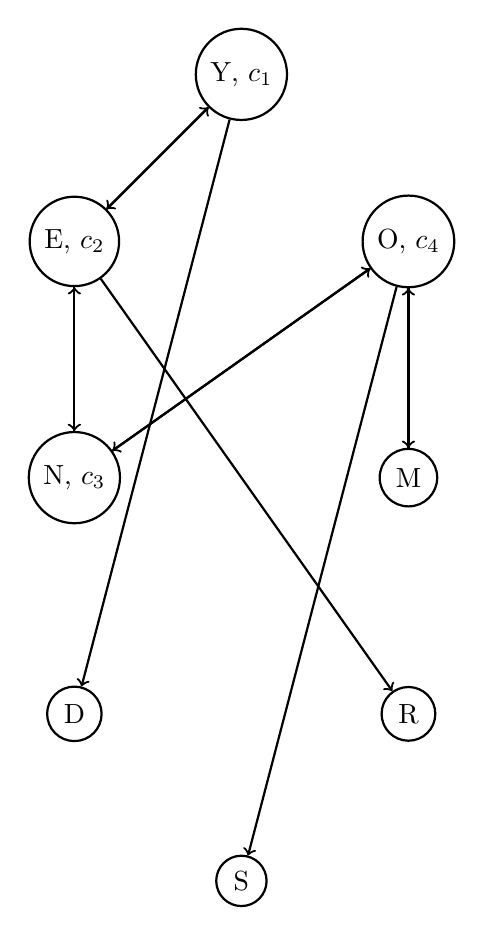
\begin{tikzpicture}[node distance={30mm}, thick, main/.style = {draw, circle}] 
    \node[main] (1)                    {Y, $c_1$}; 
    \node[main] (2) [below left  of=1] {E, $c_2$};
    \node[main] (3) [below       of=2] {N, $c_3$};
    \node[main] (4) [below right of=1] {O, $c_4$};
    \node[main] (5) [below       of=4] {M};
    \node[main] (6) [below       of=3] {D};
    \node[main] (7) [below      of=5] {R};
    \node[main] (8) [below left of=7] {S};
    \draw[->] (1) -- (2);
    \draw[->] (1) -- (6);
    
    \draw[->] (2) -- (1);
    \draw[->] (2) -- (3);
    \draw[->] (2) -- (7);
    
    \draw[->] (3) -- (2);
    \draw[->] (3) -- (4);
    
    \draw[->] (4) -- (3);
    \draw[->] (4) -- (5);
    \draw[->] (4) -- (8);
    
    \draw[->] (5) -- (4);
\end{tikzpicture} 
\end{center}


\end{itemize}
\section{A Simpler Example}
Let's experiment by solving a simple example 


\begin{center}
\begin{tabular}{ c c c c} 
   &   & T & O \\ 
 + &   & G & O \\
 \hline 
 = & O & U & T \\ 
 
\end{tabular}
\end{center}

gives us the following equations

\begin{align}
    T &= O + O       &(\mod 10) \label{eg:eq1} \\
    U &= T + G + c_1 &(\mod 10) \label{eq:eq2} \\
    O &=         c_2 &(\mod 10) \label{eq:eq3}
\end{align}

\begin{center}
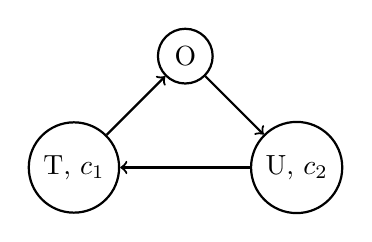
\begin{tikzpicture}[node distance={20mm}, thick, main/.style = {draw, circle}] 
    \node[main] (3)                    {O}; 
    \node[main] (1) [below left  of=3] {T, $c_1$};
    \node[main] (2) [below right of=3] {U, $c_2$};
    \draw[->] (1) -- (3);
    \draw[->] (2) -- (1);
    \draw[->] (3) -- (2);
\end{tikzpicture} 
\end{center}

\end{document}